\def\assignmenttitle{Assignment 2}
\def\assignmentdate{08-12-2011}
\def\assignmentnumber{2}

\def\mygamma{\frac{1}{\hat{y}}}
\def\mychi{\frac{1}{x}}

\documentclass[11pt]{article}
\linespread{1}

\renewcommand{\thefootnote}{\fnsymbol{footnote}}

\usepackage{geometry} % see geometry.pdf on how to lay out the page. There's lots.
\usepackage[utf8]{inputenc}
\usepackage[T1]{fontenc}
\usepackage{array}
\usepackage{amsmath,amssymb,latexsym,epic,eepic,epsfig,graphics,psfrag}
\usepackage{amsfonts}
\usepackage{graphicx,float}
\usepackage{color}
\definecolor{mygray}{RGB}{244,244,244}
\definecolor{gray}{gray}{0.5}
\definecolor{myredish}{RGB}{193,33,97}
\definecolor{grayblue}{RGB}{91,112,142}
\definecolor{myorange}{RGB}{255,134,0}
\definecolor{green}{rgb}{0,0.4,0}

\usepackage[english]{babel}

\usepackage[bottom]{footmisc}

\usepackage{fancyhdr}
\pagestyle{fancy}
\lhead{\small\textit{Assignment \assignmentnumber -- 02417 Time Series Analysis -- Anders Hørsted (s082382)}}
\rhead{\thepage}
\chead{}
\lfoot{}\cfoot{}\rfoot{}

\usepackage{subfigure}
\usepackage{pstricks}
\usepackage{pst-node}
\usepackage{wrapfig}
\usepackage{caption}
\usepackage{multirow}
%\usepackage{fouriernc}
%\usepackage[charter]{mathdesign}
\usepackage{lmodern}
\usepackage[normalem]{ulem}
\geometry{a4paper} % or letter or a5paper or ... etc
% \geometry{landscape} % rotated page geometry

\usepackage{url}


\makeatletter
\renewcommand*\env@matrix[1][*\c@MaxMatrixCols c]{%
  \hskip -\arraycolsep
  \let\@ifnextchar\new@ifnextchar
  \array{#1}}
\makeatother

\newcommand\myimp{\quad\Leftrightarrow\quad}
\newcommand\half{\frac{1}{2}}
\newcommand\myvec[1]{\mathbf{#1}}
\newcommand\mymod[1]{\ (\text{mod }#1)}
\newcommand\myreal{\mathbb{R}}
\newcommand\mynatural{\mathbb{N}}
\newcommand\myinteger{\mathbb{Z}}
\newcommand\mycomplex{\mathbb{C}}
\newcommand\myint{\text{int}}
\newcommand\norm[1]{||\,#1\,||}
\newcommand\bignorm[1]{\big|\big|\,#1\,\big|\big|}
\newcommand\seq[1]{\big\{#1\big\}}
\newcommand\smallseq[1]{\{#1\}}
\newcommand\smallseqtoinf[1]{\smallseq{#1}_{k=1}^\infty}
\newcommand\lonew{\ell^1_w}
\newcommand\lone{\ell^1}
\newcommand\ltwo{\ell^2(\mynatural)}
\newcommand\ip[2]{\langle#1,#2\rangle}
\newcommand\hilbert[1]{\mathcal{#1}}
\newcommand\uinf{u_{\infty}}
\newcommand\erf{\text{erf\,}}
\newcommand\infint{\int_{\infty}^{\infty}}
\newcommand\fpi{FPI}
\newcommand\E[1]{\text{E}[#1]}
\newcommand\Var[1]{\text{Var}[#1]}
\newcommand\Cov[1]{\text{Cov}[#1]}
\newcommand\myverb[1]{{\footnotesize\texttt{#1}}}
\newcommand\Yhat{\widehat{Y}}
\newcommand\given{\,|\,}

\usepackage[scaled]{beramono}
\usepackage{listings}
\lstset {                 % A rudimentary config that shows off some features.
    language=R,
    basicstyle=\scriptsize\ttfamily, % Without beramono, we'd get cmtt, the teletype font.
    commentstyle=\textit, % cmtt doesn't do italics. It might do slanted text though.
    keywordstyle=,
    identifierstyle=,
    framextopmargin=4pt,
    framexbottommargin=4pt,
    framexleftmargin=4pt,
    framexrightmargin=4pt,
    xleftmargin=4pt,
    xrightmargin=4pt,
    backgroundcolor=\color{mygray},
    frame=single,
    showstringspaces=false,
    captionpos=b,
    tabsize=4            % Or whatever you use in your editor, I suppose.
}

\renewcommand{\lstlistlistingname}{Code Listings}
\renewcommand{\lstlistingname}{Code Listing}

\usepackage{tabulary}
\newcolumntype{y}{>{\centering\arraybackslash}R}

\title{\assignmenttitle}
\date{\assignmentdate}
\author{Assignment \assignmentnumber\ -- 02417 Time Series Analysis -- Anders Hørsted (s082382)}
%\author{}
\date{} % delete this line to display the current date



\begin{document}

\maketitle


\section*{Question 1: Fitting to Air Pollution Data}

In this question we are going to fit sums of sines and cosines to the Air
Pollution Data given in the assignment. First a function \myverb{NOfit} that
calculates the parameters and the residuals for the fit is created.

\subsection*{Question 1.1}

The function should have the call \myverb{[x\_star, r\_star] = NOfit(t,y,n)},
but for convenience it is written to also return the design matrix $A$. The
function \myverb{NOfit} relies on \myverb{get\_A} to calculate the actual
design matrix. The function \myverb{get\_A} is used later when the fits are
plotted.

\lstinputlisting[caption={\myverb{NOfit} function to fit sine, cosines of order \myverb{n}}]{../src/NOfit.m}

\lstinputlisting[caption={Helper function \myverb{get\_A} used to generate design matrix}]{../src/get_A.m}

\subsection*{Question 1.2}

\coderemark{ex12} 

The \myverb{NOfit} function is now tested. Using the data given in the
assignment text a 3rd order cosine is fitted which gives the model. 

\begin{equation*}
    M(\myvec{x}, t) = 186.81 -44.94 \sin(\omega t) -93.43 \cos(\omega t)
\end{equation*}

To confirm the implementation of \myverb{NOfit} the residual 2-norm is checked
and it is the expected $\norm{\myvec{r^*}}_2=292.558$. Since the implementation
seems to be right, the fitted model is plotted along with the data in
figure~\ref{fig:3rd-order-fit} .\par

\begin{figure}[ht]
    \centering
    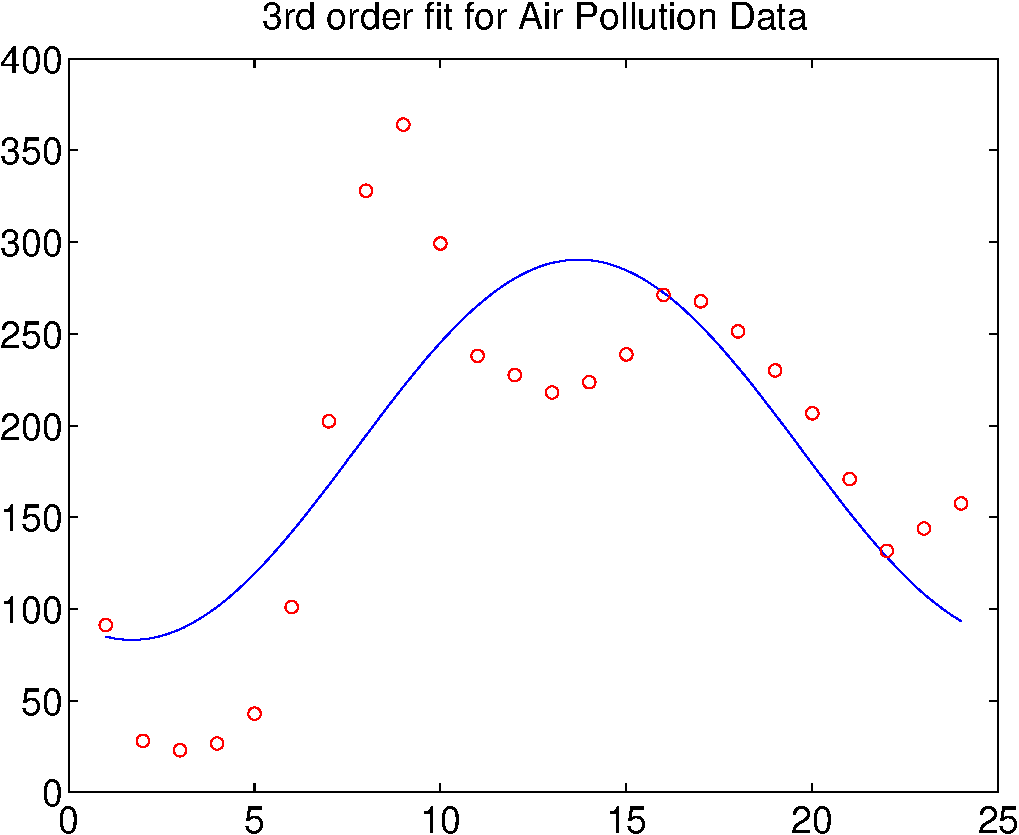
\includegraphics[width=70mm]{../media/3rd-order-fit.pdf}
    \caption{CAPTION!!!}
    \label{fig:3rd-order-fit}
\end{figure}

\subsection*{Question 1.3}

\coderemark{ex13}

The optimal order of the fit must be determined. Using the test for random
signs and the test for correlation, for the orders $n=3,5,7,9,11,13$ gives the
results shown in figure~\ref{fig:ex13}.

\begin{figure}
    \centering
    \mbox{  \subfigure{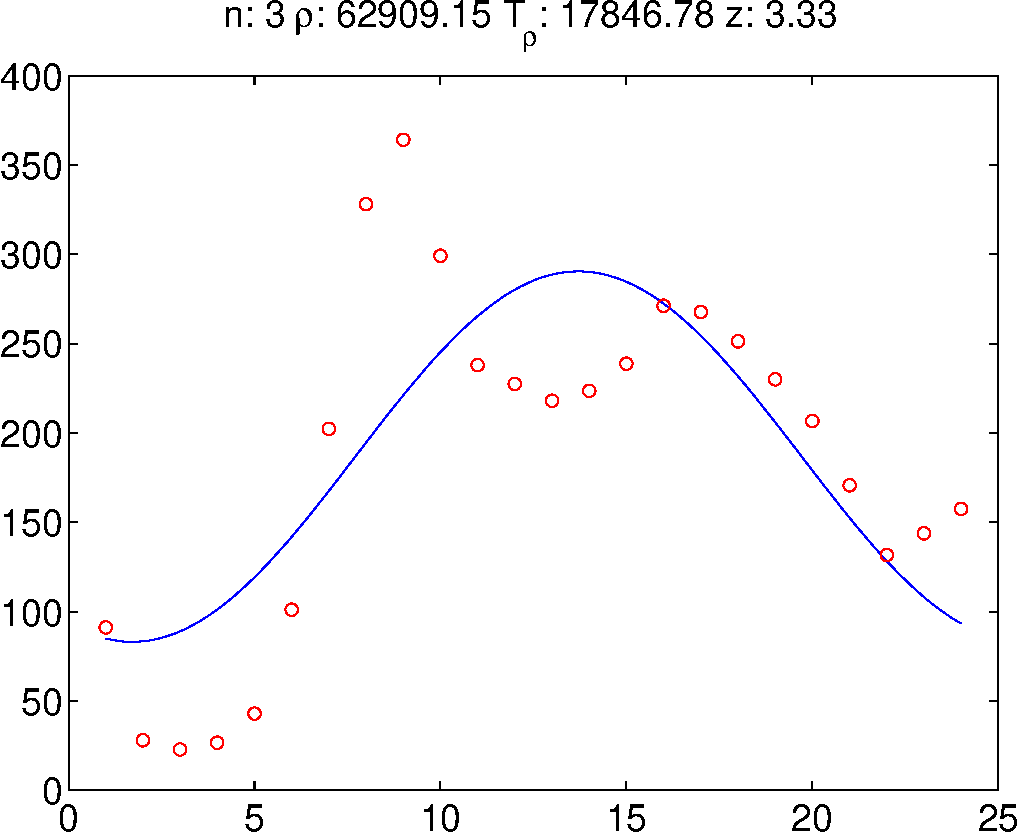
\includegraphics[width=70mm]{../media/order-determination-3.pdf}} \quad 
            \subfigure{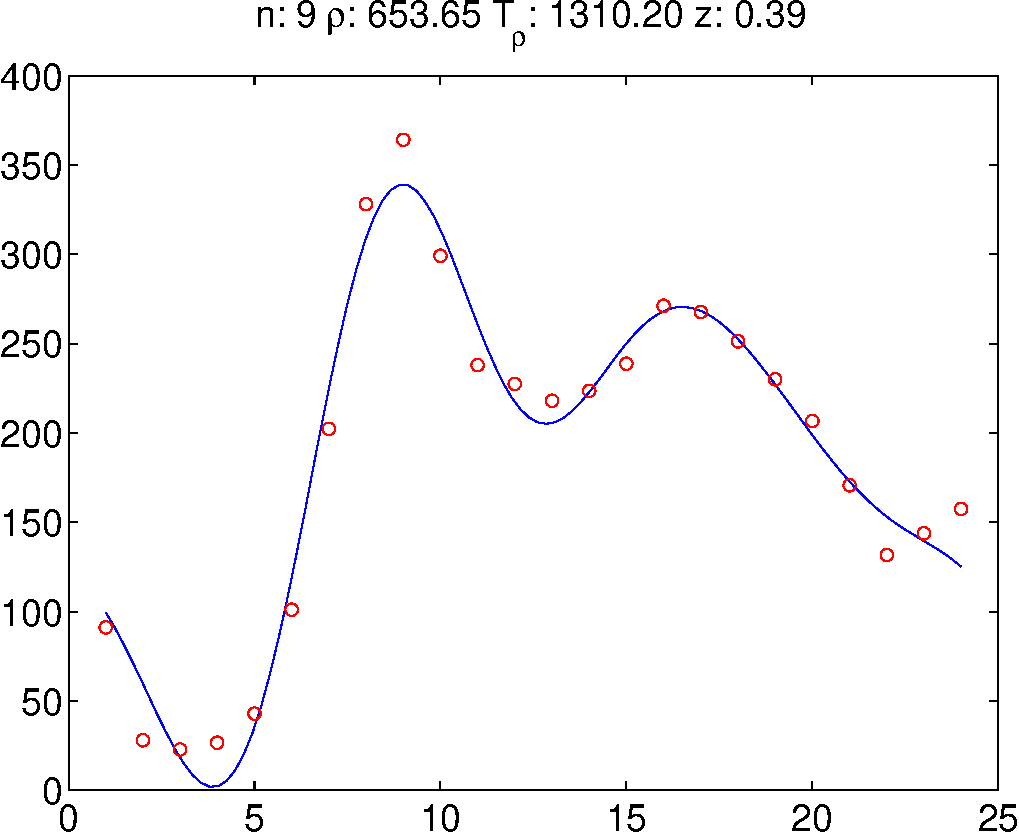
\includegraphics[width=70mm]{../media/order-determination-9.pdf}}}
    \mbox{\vspace{5mm}}
    \mbox{  \subfigure{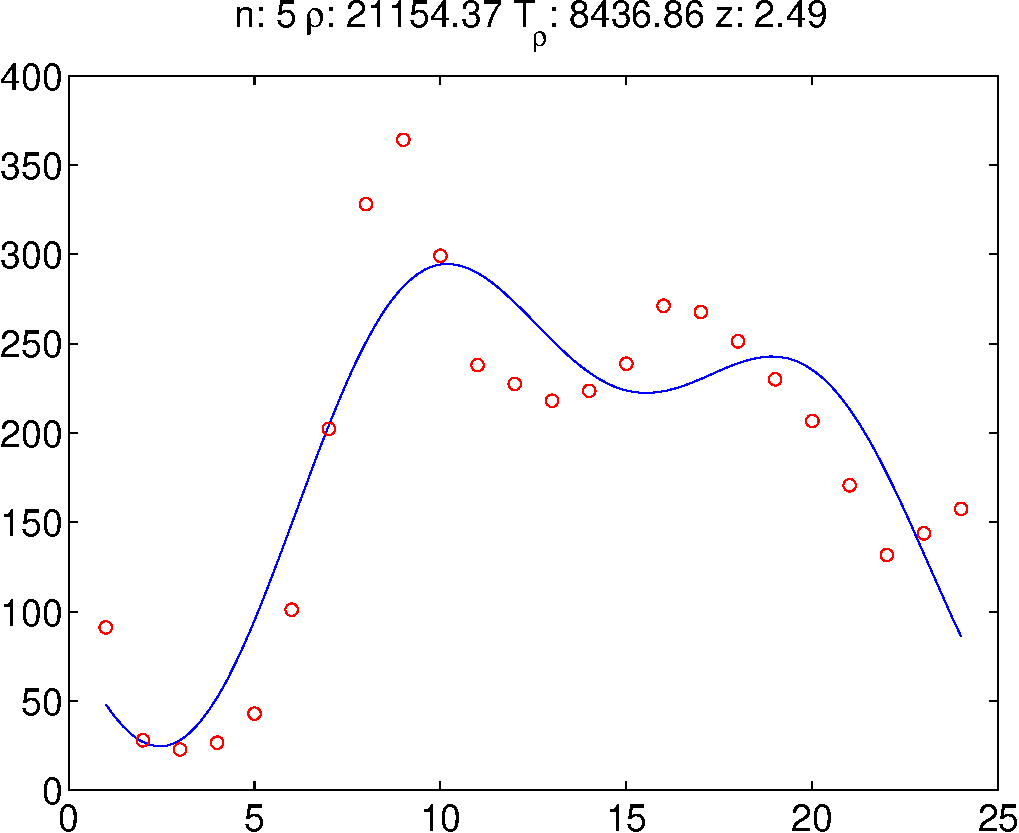
\includegraphics[width=70mm]{../media/order-determination-5.pdf}} \quad 
            \subfigure{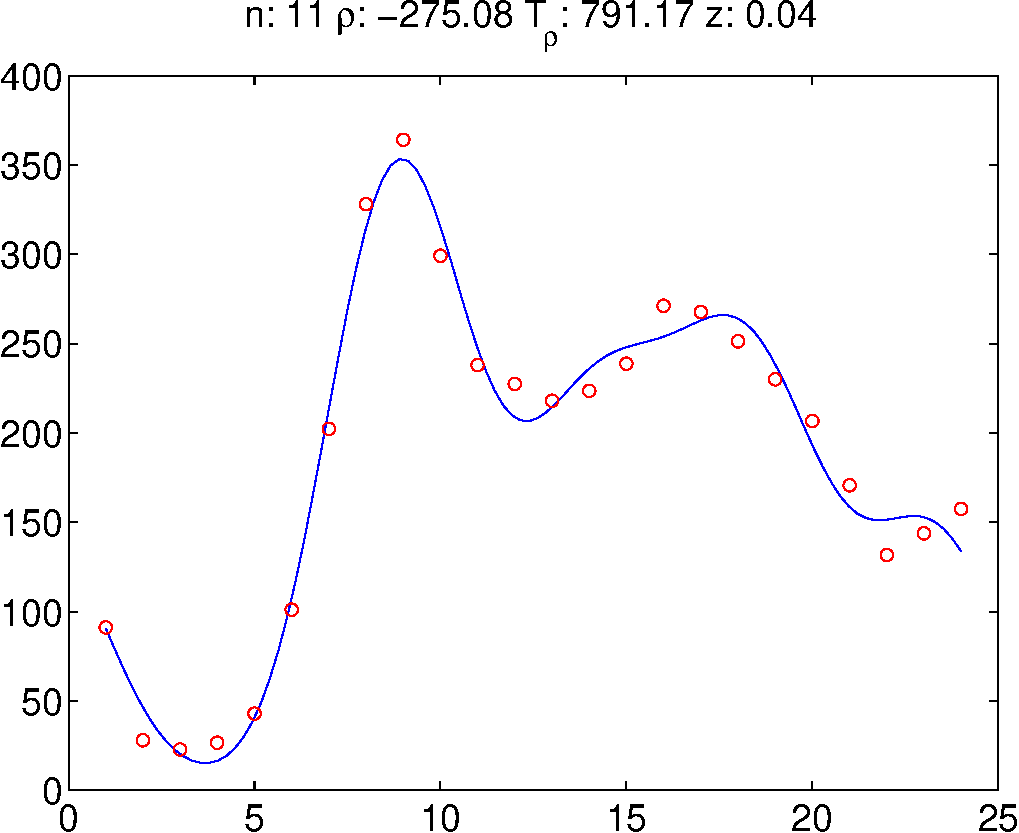
\includegraphics[width=70mm]{../media/order-determination-11.pdf}}}
    \mbox{\vspace{5mm}}
    \mbox{  \subfigure{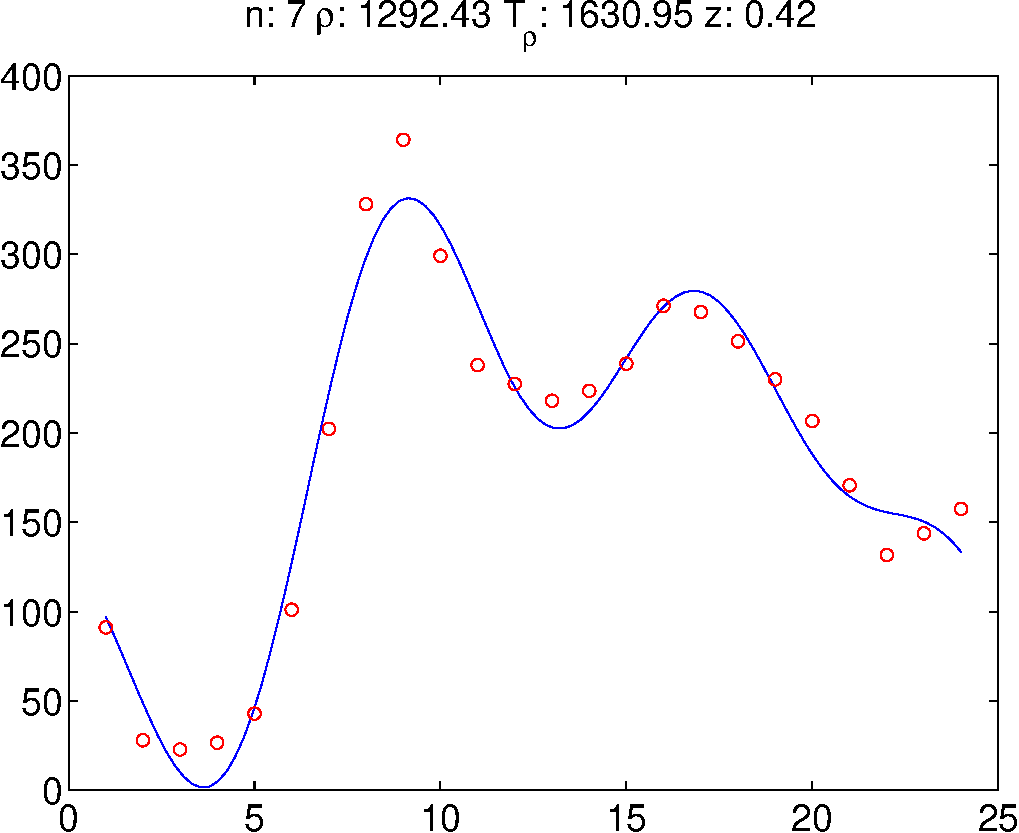
\includegraphics[width=70mm]{../media/order-determination-7.pdf}} \quad 
            \subfigure{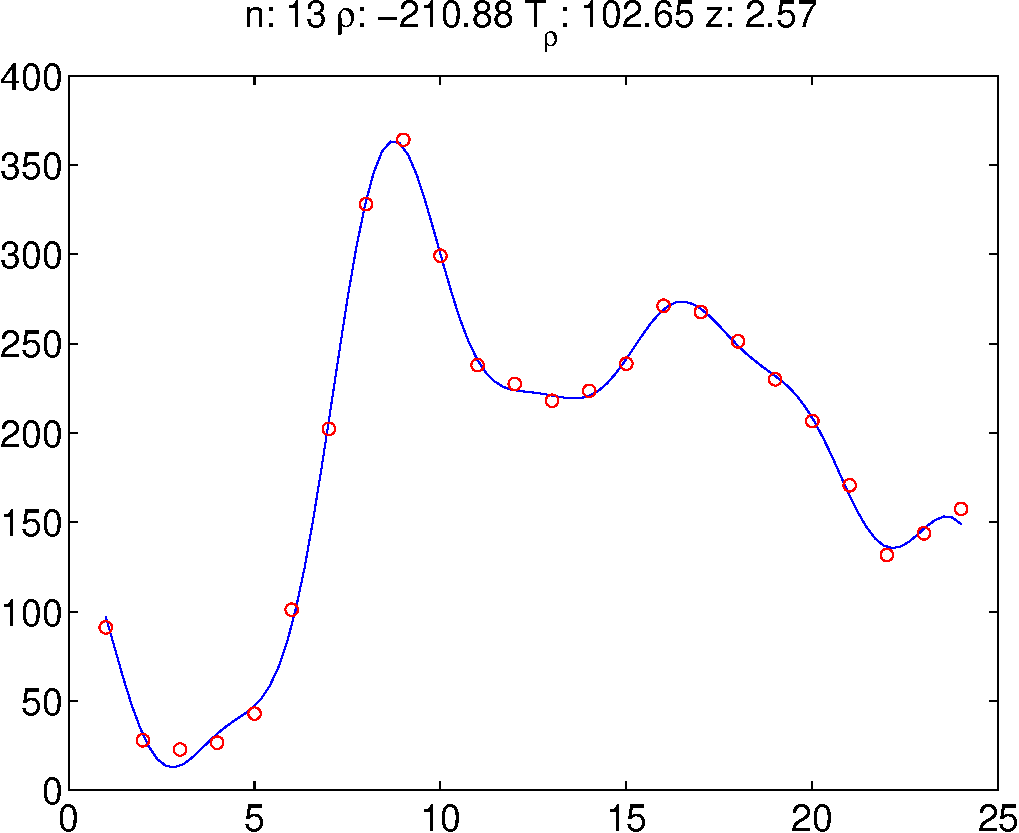
\includegraphics[width=70mm]{../media/order-determination-13.pdf}}}
    \caption{CAPTION!!!}
    \label{fig:ex13}
\end{figure}


\section*{Question 2}

In this problem a chemical reaction rate is modelled as a function of the concentration of a substrate. The predicted reaction rate is modelled as

\begin{equation*}
    \hat{y} = \frac{\theta_1 x}{\theta_2 + x}
\end{equation*}

where $x$ is the concentration and $\theta_1$ and $\theta_2$ are the parameters of interest. Given the 12 measurements of reaction rate and corresponding concentration we then model the measured reaction rate $y$ by

\begin{equation}\label{eq:ex21-base-model}
    y = \hat{y} + e
\end{equation}

where $e\sim N(0,\sigma^2)$ and $\sigma^2$ is unknown.

\subsection*{Question 2.1}

\coderemark{ex21}

First a plot of the experimental data $(x,y)$ and another plot of the inverse data $(1/x, 1/y)$ are created and shown in figure~\ref{fig:ex2-plot-data}. From the plots it do look as if a straight line could be fitted to the inverse data.

\begin{figure}[!ht]
    \centering
    \mbox{\subfigure{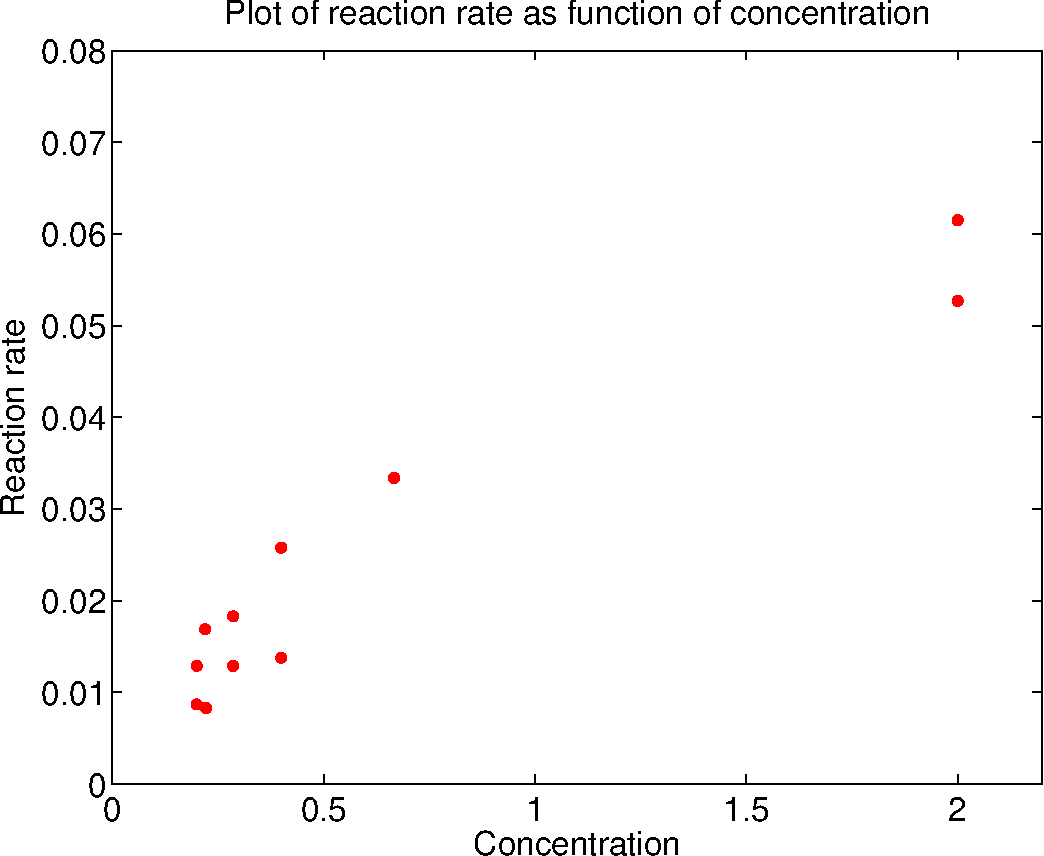
\includegraphics[width=70mm]{../media/ex21-plot.pdf}} \quad 
          \subfigure{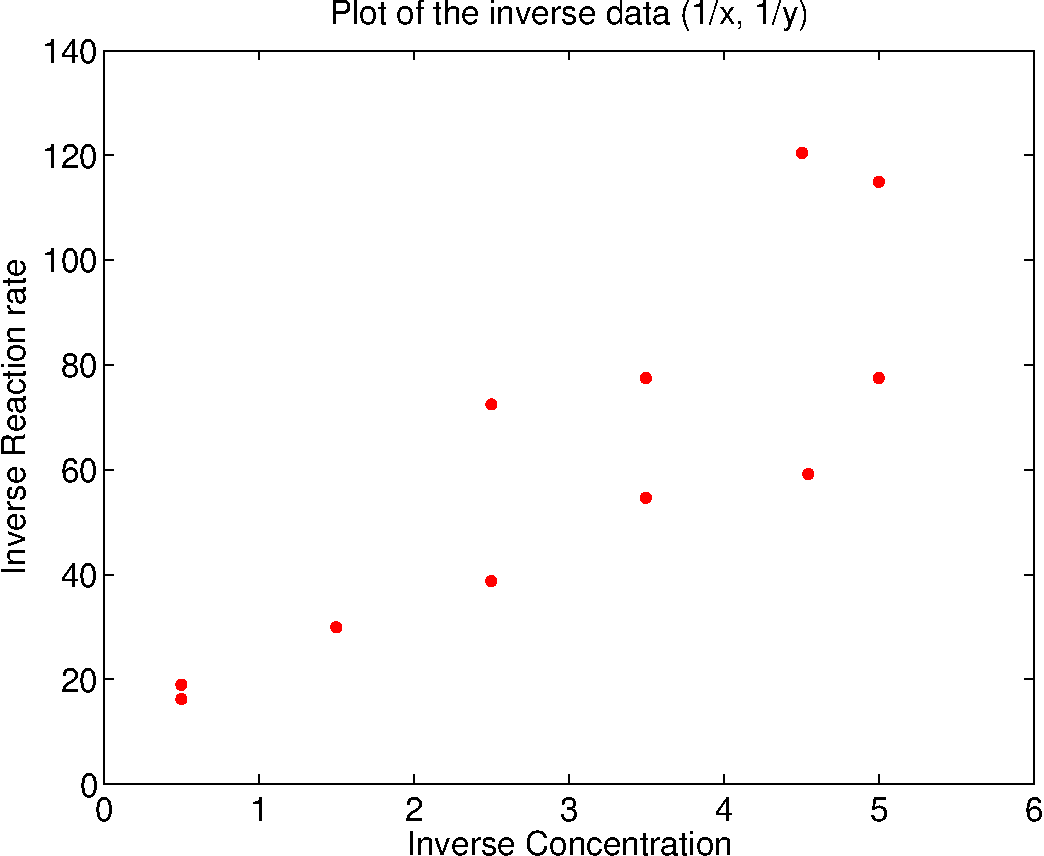
\includegraphics[width=70mm]{../media/ex21-plot-inv.pdf}}}
    \caption{Plot of experimental data $(x,y)$ and inverse data $(1/x, 1/y)$ for question 2}
    \label{fig:ex2-plot-data}
\end{figure}

Since the relationship between the inverse reaction rate and the inverse concentration could be linear, a first attempt at finding the parameters $\theta_1$ and $\theta_2$ is to look at $\mygamma$ as a function of $\mychi$. This gives

\begin{equation*}
    \mygamma = \frac{\theta_2 + x}{\theta_1x} = \frac{\theta_2}{\theta_1}\mychi + \frac{1}{\theta_1}
\end{equation*}

and by setting $\lambda_1 = \frac{1}{\theta_1}$ and $\lambda_2 = \frac{\theta_2}{\theta_1}$, we get a linear model

\begin{equation}\label{eq:ex21-linear-model}
    \mygamma = \lambda_1 + \lambda_2 \mychi
\end{equation}

We don't know $\mygamma$ but we can find an estimate for the parameters $\lambda_1$ and $\lambda_2$ by fitting $\frac{1}{y}$ linear on $\frac{1}{x}$. From the estimates of $\lambda_1$ and $\lambda_2$ we can then find $\theta_1$ and $\theta_2$. This method is implemented and shown in listing~\ref{lst:linear-params}

\lstinputlisting[label={lst:linear-params},caption={Function that finds $\theta_1$ and $\theta_2$ by fitting $\frac{1}{y}$ linear on $\frac{1}{x}$}]{../src/calc_chemical_reaction_params_linear.m}

Using the function in listing~\ref{lst:linear-params} gives the parameter estimates

\begin{equation*}
    \theta_{LS}^* \approx \begin{pmatrix} 0.14 \\ 2.54 \end{pmatrix} 

\end{equation*}

and from these parameter estimates we plot the model $\hat{y}$ along with the original data in figure~\ref{fig:data-and-linear-model}

\begin{figure}[!ht]
    \centering
    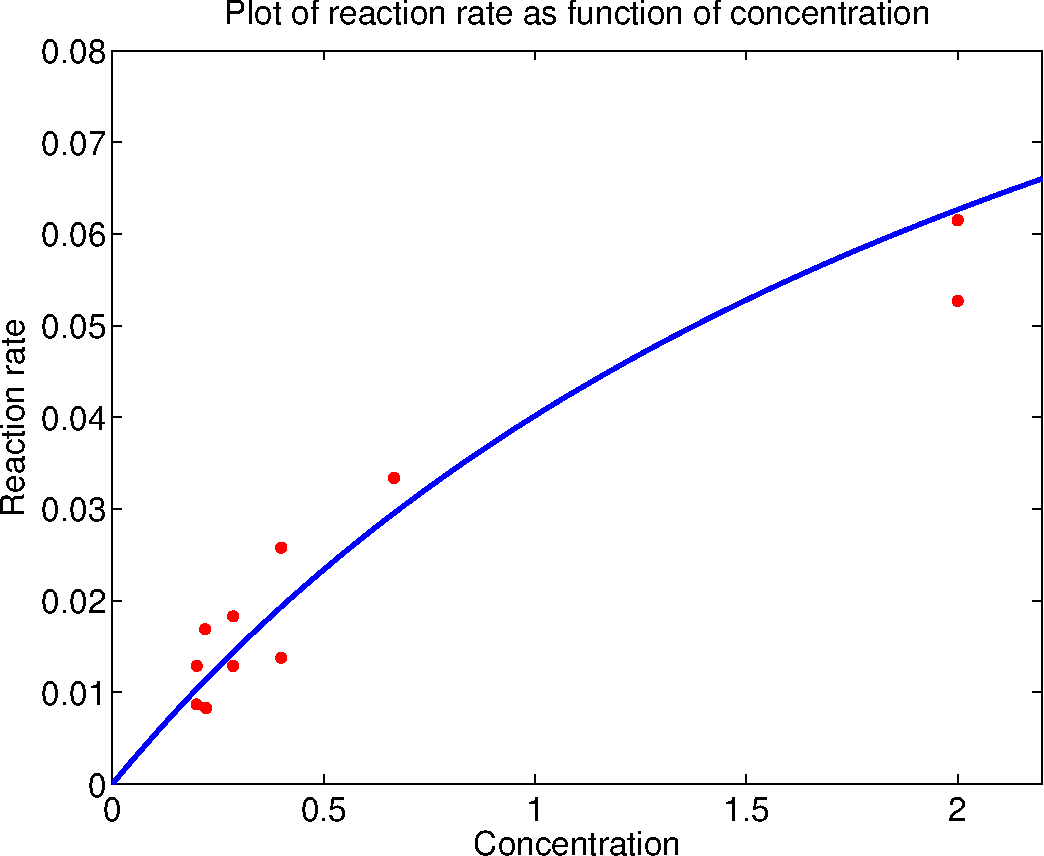
\includegraphics[width=80mm]{../media/ex21-linear-model.pdf}
    \caption{Plot of original data and the model $\hat{y}$, with parameters estimated from the linear model (\ref{eq:ex21-linear-model})}
    \label{}
\end{figure}

From the figure it is seen that the fitted model isn't explaining the data perfect. The problem is that by fitting $\frac{1}{y}$ linear on $\frac{1}{x}$ we implicitly assume that $\frac{1}{y}$ can be written as a sum of a linear model of $\frac{1}{x}$ and an gaussian error term. This is the same as assuming that $\frac{1}{y}$ is normal distributed, but from our original model (\ref{eq:ex21-base-model}) we get that $y$ is normal distributed with mean $\hat{y}$ and variance $\sigma^2$. We therefore found the parameter estimate $\theta_{LS}^*$ by assuming that the inverse of a normal distributed variable, is also normal distributed. This isn't correct and as a result we found that the fit wasn't perfect.


\subsection*{Question 2.2}

In this question the parameters $\theta$ is found by solving the non-linear least squares problem.

\begin{equation*}
    \phi(\theta) = \half\sum_{i=1}^n \norm{y_i - f(\theta; x_i)}_2^2
\end{equation*}

First a contour plot of $\phi(\theta)$ is created and $\theta_{LS}^*$ is shown with a dot in the plot. The contour plot is shown in figure~\ref{fig:ex22-contour-linear} and it looks as if there are values for $\theta$ that gives smaller values for $\phi(\theta)$ than $\theta_{LS}^*$.

\begin{figure}[ht]
    \centering
    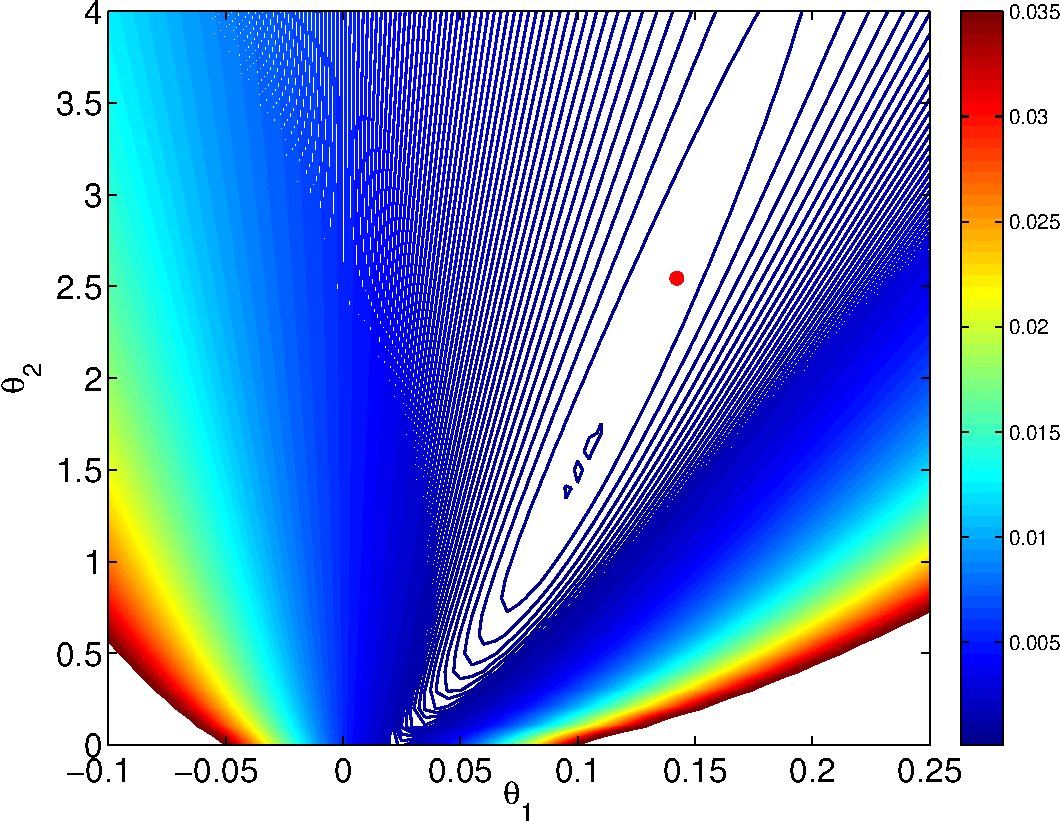
\includegraphics[width=70mm]{../media/ex22-contour-linear.pdf}
    \caption{CAPTION XXX}
    \label{fig:ex22-contour-linear}
\end{figure}

To find an better estimate than $\theta_{LS}^*$, a nonlinear least squares method is used instead of the linear least squares method from the previous question. Specifically the Marquardt algorithm is used to find $\theta^*$ {\textcolor{red}{COMMENT ON ALGORITHM!!!}}.

By running the marquardt function the parameter estimate $\theta^*$ is found as

\begin{equation*}
    \theta^* \approx \begin{pmatrix} 0.10 \\ 1.51 \end{pmatrix} 

\end{equation*}

and estimates for $\hat{\sigma}^2$ and $\text{Cov}[\theta^*]$ is found as

\begin{equation*}
    \hat{\sigma}^2 \approx 9.54e\mbox{-}06 
, \quad \text{Cov}[\theta^*] \approx \begin{bmatrix} 0.000111 & 0.00275 \\ 0.00275 & 0.0742 \end{bmatrix}
\end{equation*}

From $\hat{\sigma}^2$ and $\text{Cov}[\theta^*]$ a 95\% confidence intervals for $\theta^*$ can be found which gives

\begin{equation*}
    \text{Conf}_{95\%}(\theta_1^*) \approx [0.0804; 0.122], \quad \text{Conf}_{95\%}(\theta_2^*) \approx [0.98; 2.05]
\end{equation*}

The optimal estimate $\theta^*$ is now plotted in a contour plot of $\phi(\theta)$ and is shown in figure~\ref{fig:ex22-contour-marquardt}. From the figure it looks as if the new estimate gives a lower value for $\phi(\theta)$, than the estimate from the previous question. 

\begin{figure}[ht]
    \centering
    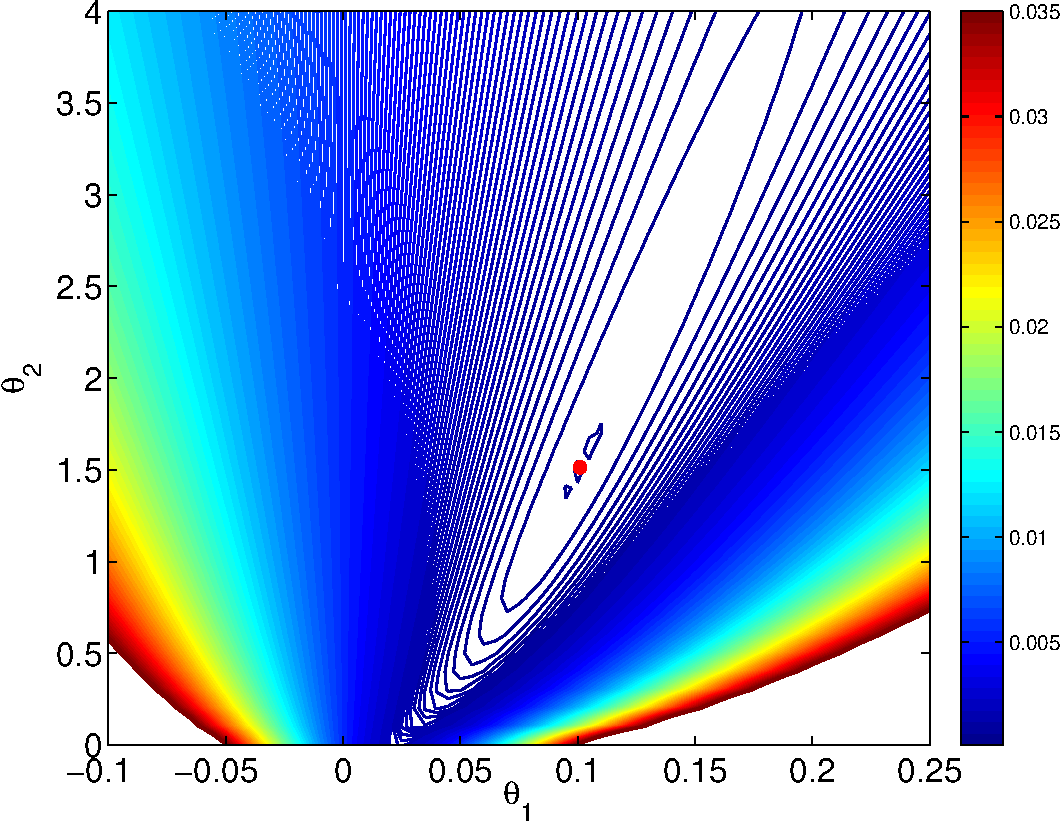
\includegraphics[width=70mm]{../media/ex22-contour-marquardt.pdf}
    \caption{CAPTION XXX}
    \label{fig:ex22-contour-marquardt}
\end{figure}

To better visualize the improvement the Michaelis-Menten model is now plotted for both $\theta_{LS}^*$ and $\theta^*$ along with the measured data. The plot is found in figure~\ref{fig:ex22-models} and the model with $\theta^*$ as parameters seems to fit the data best.

\begin{figure}[ht]
    \centering
    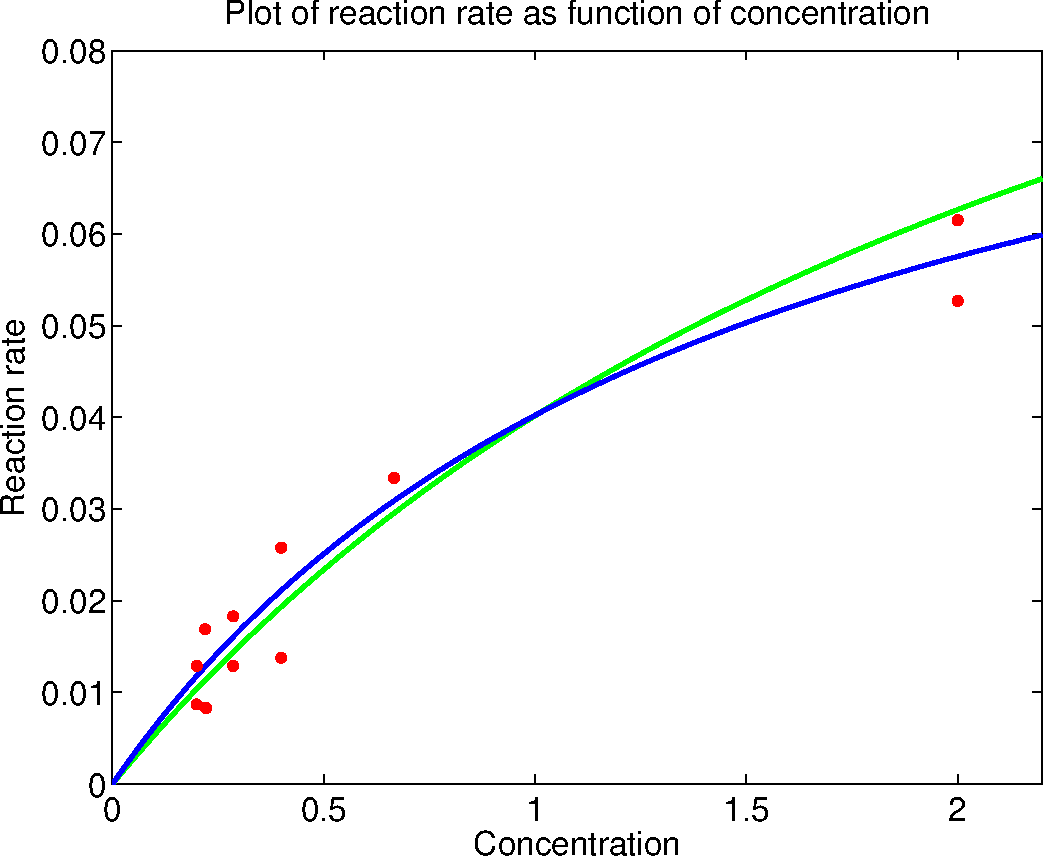
\includegraphics[width=70mm]{../media/ex22-models-with-data.pdf}
    \caption{CAPTION XXX}
    \label{fig:ex22-models}
\end{figure}


\section*{Question 2.3}

We continue to work with the chemical reaction used in question 2.1 and 2.2, but instead of measurements of reaction rate and concentration, we now have measurements of concentrations $x_i$ at different times $t_i$. Denoting the real concentration at time $t$ as $x(t)$ the measured concentration is modelled as
\begin{equation*}
    y(t_i) = \hat{y}(\theta; t_i) + e
\end{equation*}

where $e\sim N(0, \sigma^2)$ and $\hat{y}(\theta; t_i)=x(t_i; \theta)$ is the concentration predicted by

\begin{equation}\label{eq:ex23-ode}
    \frac{dx(t)}{dt} = -\frac{\theta_1 x(t)}{\theta_2 + x(t)}, \quad x(0) = 10.0
\end{equation}

The parameters $\theta$ should now be estimated by

\begin{equation}\label{eq:ex23-min}
    \min_\theta\:\phi(\theta) = \half\sum_{i=1}^n \norm{y(t_i) - \hat{y}(\theta;t_i)}^2_2
\end{equation}

using the measurements in \myverb{MMBatchData.mat}. The data is plotted in figure~\ref{fig:ex23-data}

\begin{figure}[ht]
    \centering
    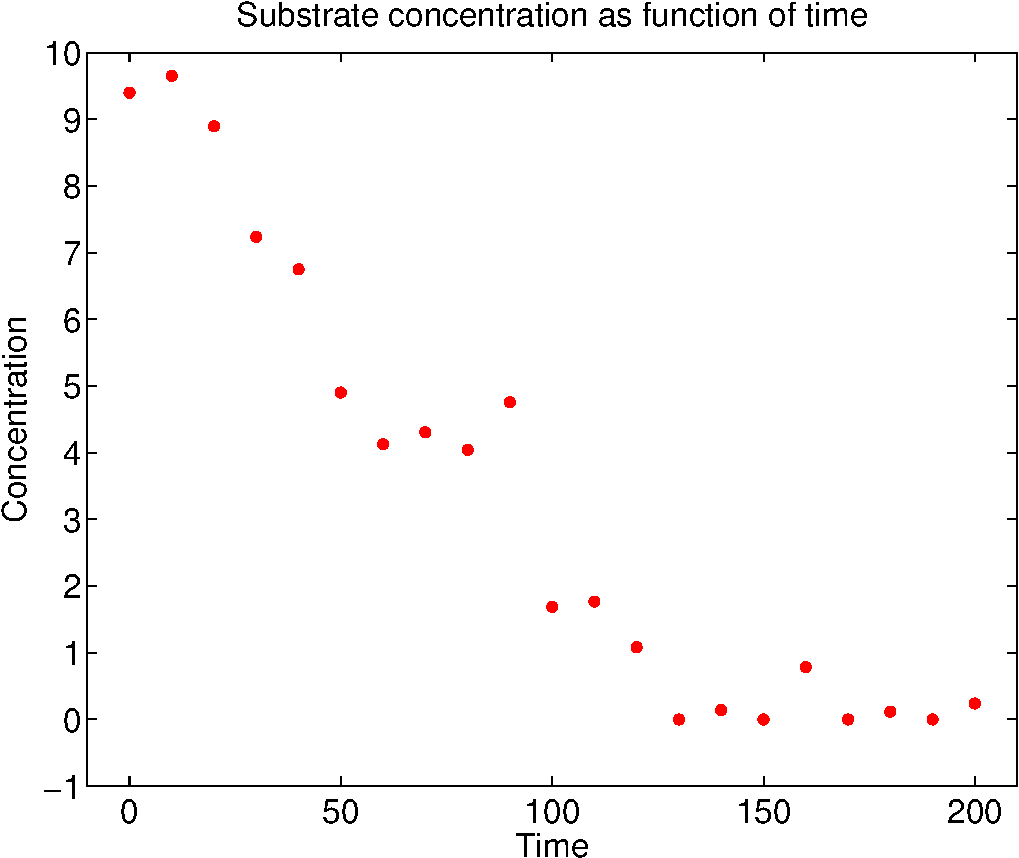
\includegraphics[width=80mm]{../media/ex23-data.pdf}
    \caption{CAPTION XXX}
    \label{fig:ex23-data}
\end{figure}

To actually estimate $\theta$ a Matlab function that computes $\hat{y}(\theta; t_i)$ for a given $\theta$ and all $t_i$, is implemented and shown in listing~\ref{lst:ex23-yhat}. The function takes a vector \myverb{t} containing all $t_i$s and another vector \myverb{p} that is the parameter $\theta$. Using the Matlab function \myverb{ode45} the solution of (\ref{eq:ex23-ode}) is found for all $t_i$, and since $\hat{y}=x$ we can directly return the solution obtained from \myverb{ode45}

\lstinputlisting[label=lst:ex23-yhat,caption={Function to compute $\hat{y}(\theta,t_i)$, for a given $\theta$ and all $t_i$}]{../src/ex23_yhat.m}

We are now able to compute $\hat{y}(\theta; t_i)$ and therefore we can also compute $\phi(\theta)$ for different values of $\theta$. Therefore a contour plot of $\phi(\theta)$ can be created. The contour plot is shown in figure~\ref{fig:ex23-contour}. From the plot there seems to be a minimum near (0.1, 1).

\begin{figure}[ht]
    \centering
    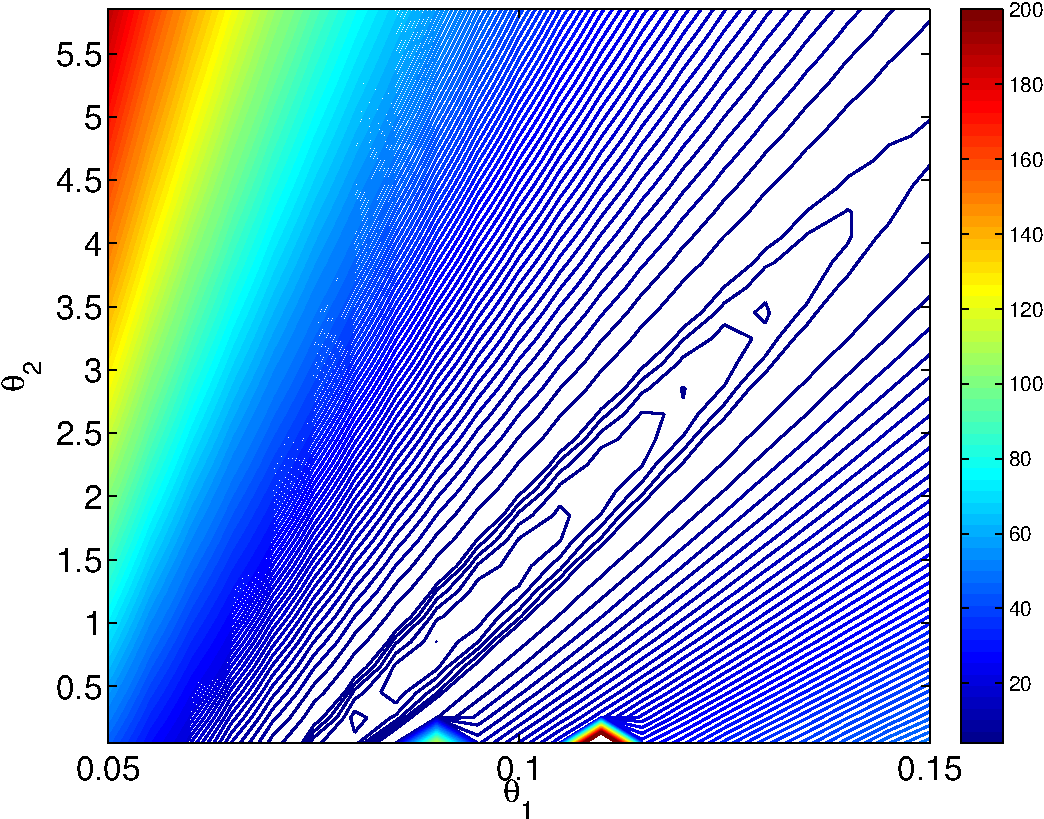
\includegraphics[width=80mm]{../media/ex23-contour.pdf}
    \caption{CAPTION XXX}
    \label{fig:ex23-contour}
\end{figure}

To actually find a minimum for $\phi(\theta)$ a nonlinear least squares algorithm is used. To get good performance we need to supply the least squares function with the derivative of $\phi(\theta)$. From (\ref{eq:ex23-min}) we get that 

\begin{equation*}
    \frac{\partial\phi(\theta)}{\partial\theta}=-\sum_{i=1}^n\frac{\partial\hat{y}(\theta; t_i)}{\partial\theta}
\end{equation*}

A function that calculates $\frac{\partial}{\partial\theta}\hat{y}(\theta;t_i)$ (and $\hat{y}(\theta;t_i)$) for all $t_i$ is therefore implemented and shown in listing~\ref{lst:ex23-yhatdot}.

\lstinputlisting[label=ex23-yhatdot,caption={CAPTION!!!}]{../src/ex23_z.m}

The implementation is based on page 11-17 in the slides for lecture 12. The implementation utilizes the fact that since $\hat{y}=x$ we have that (using the notation of the slide) $S_\theta(t) = \frac{\partial}{\partial\theta}\hat{y}(\theta; t)$. By calculating $z$ (as defined on slide 16) we get excatly the information we need to run a non-linear least squares method.

The parameters $\theta$ is now found by using the \myverb{marquardt} method from the IMM optimbox with the settings \myverb{tau=1e-3}, \myverb{tolg=1e-7}, \myverb{tolx=1e-12} and \myverb{maxeval=100}. The function uses 35 iterations to find the parameters

\begin{equation*}
    \theta \approx \begin{pmatrix} 0.09 \\ 0.77 \end{pmatrix} 

\end{equation*}

When the parameters are found, $\hat{\sigma}^2$ and $\text{Cov}[\theta]$ can be estimated, which gives

\begin{equation*}
    \hat{\sigma}^2 \approx 0.21 
, \quad \text{Cov}[\theta] \approx \begin{bmatrix} 7.28e\mbox{-}05 & 0.00445 \\ 0.00445 & 0.293 \end{bmatrix}
\end{equation*}

Using $\hat{\sigma}^2$ and $\text{Cov}[\theta]$, confidence intervals for the parameter estimates can be calculated, which gives

\begin{equation*}
    \text{Conf}_{95\%}(\theta_1) \approx [0.0725; 0.106], \quad \text{Conf}_{95\%}(\theta_2) \approx [-0.29; 1.83]
\end{equation*}


\pagebreak
\renewcommand\thesection{\Alph{section}}


\section{Appendices}

All \matlab\ source code is included in the appendices. All the source code
including the LaTex code used for the report can also be found at
\url{https://github.com/alphabits/dtu-fall-2011/tree/master/02610/assignment-2}.

\subsection{Question 1.2}\label{app:ex12}
\lstinputlisting[caption={ex12.m}]{../src/ex12.m}

\subsection{Question 1.3}\label{app:ex13}
\lstinputlisting[caption={ex13.m}]{../src/ex13.m}

\subsection{Question 2.1}\label{app:ex13}
\lstinputlisting[caption={ex21.m}]{../src/ex21.m}

\subsection{Helper functions}\label{app:helpers}
\lstinputlisting[caption={plot\_fit.m}]{../src/plot_fit.m}
\lstinputlisting[caption={plot\_fit\_with\_res\_analysis.m}]{../src/plot_fit_with_res_analysis.m}

\pagebreak
\begin{thebibliography}{9}

\bibitem{hm}
  Henrik Madsen,
  \emph{Time Series Analysis}.
  Chapman \& Hall/CRC,
  1st Edition,
  2008.

%\bibitem{taleb}
%  Nassim Nicholas Taleb,
%  \emph{The Black Swan}.
%  Random House Trade Paperbacks
%  2nd Edition,
%  2010.

\end{thebibliography}


\end{document}
